\documentclass{beamer}
\usepackage[utf8]{inputenc}

\usetheme{CambridgeUS}
\usecolortheme{default}
\usepackage{tikz}
\usepackage{caption}
\captionsetup{font=scriptsize,labelfont=normalsize}
\captionsetup[figure]{labelformat=empty}
\setbeamertemplate{caption}{\raggedright\insertcaption\par}

%------------------------------------------------------------
%This block of code defines the information to appear in the
%Title page
\title[Master Thesis] %optional
{Advancing Packet-Level Predictions with Transformers}
\date{September 1, 2022}
\author[Siddhant Ray] % (optional)
{Siddhant Ray}

\institute[ETH Zürich] % (optional)
{
  Dept. of Information Technology and Electrical Engineering(D-ITET) \\
  ETH Zürich
}



%\date[September 2022] % (optional)

\titlegraphic{
    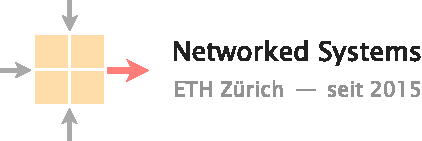
\includegraphics[width=2cm]{figures/nsg_logo.pdf}
    \hspace{2cm}
     
\includegraphics[width=2cm]{figures/eth_logo.pdf}
}

%End of title page configuration block
%------------------------------------------------------------



%------------------------------------------------------------
%The next block of commands puts the table of contents at the 
%beginning of each section and highlights the current section:

%\AtBeginSection[]
%{
%  \begin{frame}
 %   \frametitle{Table of Contents}
 %   \tableofcontents[currentsection]
 % \end{frame}
%}
%------------------------------------------------------------


\begin{document}

%The next statement creates the title page.
\frame{\titlepage}


%---------------------------------------------------------
%This block of code is for the table of contents after
%the title page
%\frametitle{Table of Contents}
%
%end{frame}
%---------------------------------------------------------


\section{Motivation}

%---------------------------------------------------------
%Changing visivility of the text
\begin{frame}
\frametitle{Why Transformers?}

\begin{itemize}
    \item<1-> Efficient learning with attention mechanism
    \item<1-> Large datasets available to learn from
    \item<2-> State-of-art for sequence learning 
     \item<2-> Network packet data is a sequence
\end{itemize}
\end{frame}

\begin{frame}
\frametitle{Why Transformers?}

We present the Network Traffic Transformer(NTT):
\pause

 \begin{itemize}  
    \item<1-> Pre-train on network packet data (few times)
    \item<1-> Fine-tune for specific tasks (many times)
\end{itemize}

\begin{figure}[!hbt]
  \begin{center}
    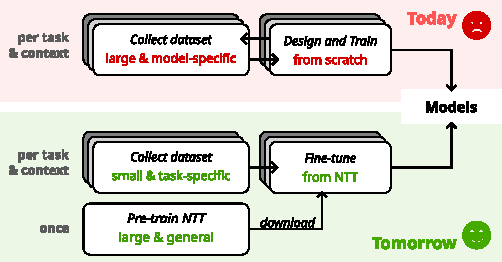
\includegraphics[scale=0.8]{figures/vision.pdf}
    \caption{Pre-train today, fine-tune and re-use tomrrow}
    \label{fig:vision}
  \end{center}
\end{figure}
    
    
\end{frame}

%---------------------------------------------------------


%---------------------------------------------------------
%Example of the \pause command
\begin{frame}
\frametitle{Success in NLP and CV}
BERT:

add small list
\pause

Vision Transformer:

add small list


\end{frame}
%---------------------------------------------------------

\section{Design}

%---------------------------------------------------------
%Highlighting text

\begin{frame}
\frametitle{NTT architecture}

Feature selection for NTT's input data:
\pause 
\begin{itemize}
    \item<1-> \alert{Relative timestamp:} To learn sequence order
    \item<1-> \alert{End-to-end delay:} To learn network state information
    \item<1-> \alert{Packet size:} To learn packet state information
\end{itemize}

\end{frame}

\begin{frame}
\frametitle{NTT architecture}

\begin{figure}[!hbt]
  \begin{center}
    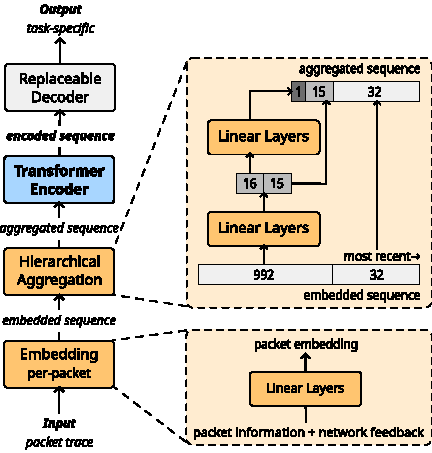
\includegraphics[scale=0.8]{figures/architecture_ntt.pdf}
    \caption{The Network Traffic Transformer (NTT) with
        an embedding layer, % for feature extraction,
        an aggregation layer, and
        a transformer encoder.}
    \label{fig:ntt}
  \end{center}
\end{figure}
\end{frame}

\begin{frame}
\frametitle{NTT architecture}

NNT's learning strategies: 
\pause 
\begin{itemize}
    \item<1-> \alert{Masking delays:} Reconstruct masked values to sequence structure
    \item<1-> \alert{Variable masking:} Robust learning with multi-positional masks
    \item<1-> \alert{Aggregating inputs} To learn and scale to larger sequences
\end{itemize}
\end{frame}



\begin{frame}
\frametitle{Pre-training setup}


\begin{figure}[h]
  \begin{center}
    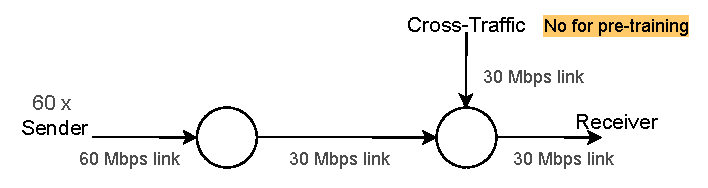
\includegraphics[scale=0.8]{figures/simple_topo.pdf}
    \caption{Initial topology for data generation}
    \label{fig:topo}
  \end{center}
\end{figure}
 
 \pause

Show plots on pre-training?? \pause

Show key insights.

\end{frame}



%---------------------------------------------------------

\section{Evaluation}

%---------------------------------------------------------
%Two columns
\begin{frame}
\frametitle{Understanding NTT's Performance}



\begin{columns}
\column{0.5\textwidth}
Use two columns 
\column{0.5\textwidth}
only if needed.
\end{columns}
\end{frame}


\begin{frame}
\frametitle{Understanding NTT's Performance}

Show tables from thesis \pause 

Show plots thesis \pause

Write key insights.

\end{frame}

%---------------------------------------------------------

\section{Future}

\begin{frame}
\frametitle{Improve NTT}

\begin{itemize}
    \item<1-> Learn more features/ scale to more complexity
    \item<2-> Federated learning/ sharing/ data privacy
    \item<3-> Continual learning/ re-training
\end{itemize}
\end{frame}

\section{Comments}
\begin{frame}
\frametitle{Time for questions}

\end{frame}



\end{document}